\section{Classification Models} \label{sec:impl/clf_models}

All classification models detailed below were implemented in Python using toolsets provided by the Pytorch Deep Learning Library \cite{paszke2019}. This allows for higher abstraction when designing model architectures, without having to manually implement backpropagation, optimizers, activation functions and other standard machine learning concepts. Leaving these implementations to the experts offer the promise that the training process may be GPU accelerated and optimized for computing efficiency.

While some models could be trained on a mere laptop CPU, all the deeper architectures were trained using a cloud computing instance provided by Amazon Web Services. The instance used had four Intel Xeon Cascade Lake P-8259L processors, 16GiB memory and a  Nvidia T4 Tensor Core GPU with 16GiB graphics memory.

\subsection{Architecture}

The architecture of a neural network is what defines the hypothesis space in which predictions may be made from a given input. Deeper networks can encapsulate more complex features of a dataset, at the increased risk of overfitting features which do not generalize well outside of the training data. For this thesis, the selection of model architectures is inspired by a review of deep learning for \acrshort{tsc} presented by \textcite{fawaz2018}. Although an overview is provided in the following subsections, a comprehensive list of all model architectures can be studied in appendix \ref{app:arch_details}.

All models aim to be fully end-to-end and able to classify multivariate time series of undefined dimension. Input time series are multivariate in their data channels (e.g. pupillary, coordinate and \acrshort{ebr} data channels) and temporal. Their dimension is therefore defined by its length in time, sampling frequency and number of data channels. 

\newpage
\subsubsection{\acrlong{mlp}}

\begin{figure}[h]
    \centering
    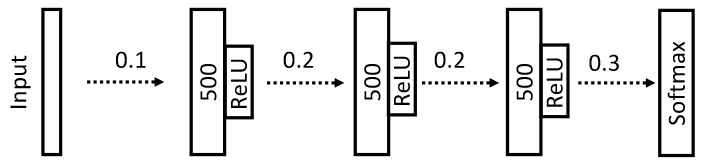
\includegraphics[width=\textwidth]{figures/impl_MLP.png}
    \caption{\acrlong{mlp} architecture. }
    \source{\textcite{wang2016}}
    \label{fig:impl_MLP}
\end{figure}

First up is the traditional and well-known \acrfull{mlp}. Being an integral part of deep learning history, it is a natural inclusion as a baseline by which other architectures may be compared. This particular implementation, first proposed for \acrshort{tsc} by \textcite{wang2016}, is presented in figure \ref{fig:impl_MLP}. It is composed of four layers where all neurons are connected to activations from neurons of the previous layer. The three hidden layers between input and output are each composed of 500 neurons with \acrshort{relu} as the activation function. Between all layers is a dropout operation with dropout rates ranging from 10\% to 30\%. The input layer takes in all samples in one time segment, from all data channels. With input segments of length 256, the layers of this model contain $1,015,504$ parameters. Outputs from the last hidden layer is passed through a softmax function, such that the model output is a probability distribution over all classes that sum to one.

Since all layers in a \acrshort{mlp} are fully connected, any temporal invariance between time-consecutive samples in the data is lost. This is because all input neurons to every layer is weighted independently from one another, such that the time-dimension from input samples is essentially ignored. Since temporal invariance is an important factor for \acrshort{tsc}, the \acrshort{mlp} is likely a sub-optimal alternative to other deep learning architectures. 

\newpage
\subsubsection{\acrlong{fcn}}

\begin{figure}[h]
    \centering
    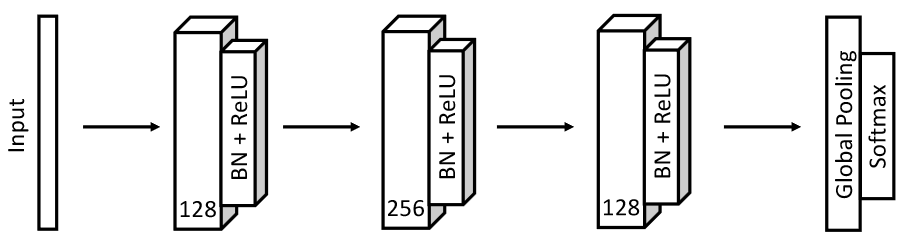
\includegraphics[width=\textwidth]{figures/impl_FCN.png}
    \caption{...}
    \source{\textcite{wang2016}}
    \label{fig:impl_FCN}
\end{figure}

The second architecture presented is a form for \acrshort{cnn} for \acrshort{tsc}, as described in section \ref{sec:bt/DNN}. Like the \acrshort{mlp}, this \acrfull{fcn} implementation was proposed by \textcite{wang2016}, and is presented in figure \ref{fig:impl_FCN}. It is composed of three convolutional blocks, where each block is appended with a batch normalization layer which is passed through a \acrshort{relu} activation function. Layers have 128, 256 and 128 convolutional filters, with filter lengths of eight, five and three, respectively. Even though this architecture have the same layer depth as the \acrshort{mlp}, its convolutional nature allows for fewer total parameters, at $268,292$. Output from the last layer is fed into a global average pooling layer that collapses the entire time dimension to a single value for every filter. These values are subsequently passed onto a fully connected classifier activated by a softmax function. Similar to the \acrshort{mlp}, the output is therefore a probability distribution that sums to one.

% Since the learned parameters of a \acrshort{cnn} is merely the internal weights of all convolutional filters, temporal invariance is achieved because 

Contrary to a \acrshort{mlp} architecture, the convolutional nature of the \acrshort{fcn} allow for temporal invariance. The resulting model can therefore recognize relations in time, as opposed to raw sample inputs. Another advantage the \acrshort{fcn} is an invariance in the total number of parameters. Since the global average pooling layer collapses the time dimension, parameters are only dependent on the number of layers and filters, which is constant. This invariance allows for the use of a transfer learning approach, since the learned convolutional filter weights will learn features which is independent of segment length.

\newpage
\subsubsection{\acrlong{mcdcnn}}

\begin{figure}[h]
    \centering
    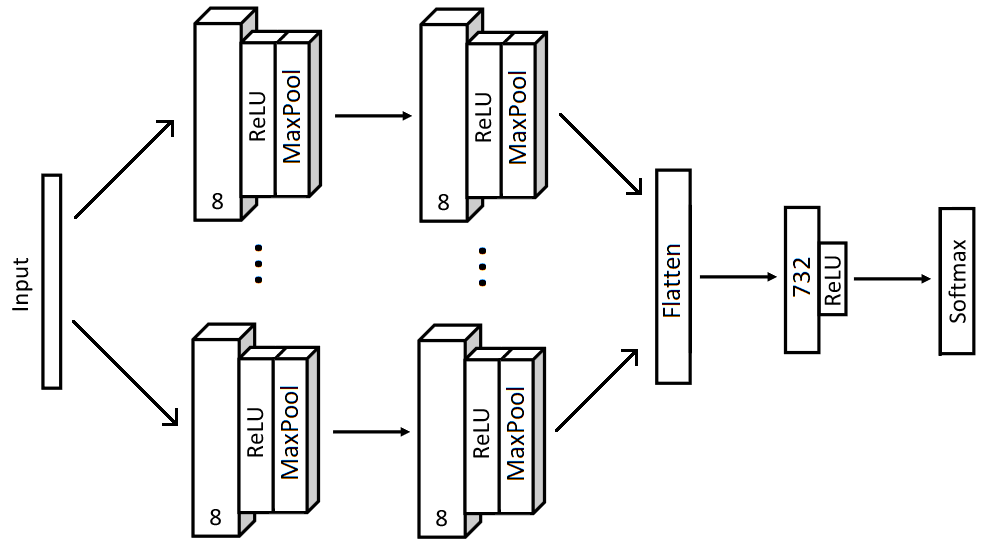
\includegraphics[width=\textwidth]{figures/impl_MCDCNN.png}
    \caption{...}
    \label{fig:impl_MCDCNN}
\end{figure}

The \acrfull{mcdcnn} is in some ways a blend of a \acrshort{mlp} and a \acrshort{fcn}. It was originally proposed and validated by \textcite{zheng2014}, and was expected to perform especially well on multivariate time series datasets. As is illustrated in figure \ref{fig:impl_MCDCNN}, it consists of two convolutional stages with eight filters of length five. Following the convolutions is a \acrshort{relu} activation function and a max pooling operation. Uniquely, these convolutional stages are all applied in parallel before their outputs are flattened and passed to a fully connected layer with 732 neurons, again with \acrshort{relu} as its activation function. This model contains slightly more parameters than the \acrshort{fcn}, at $378,632$. Output from the fully connected layer is equal to the number of classes to be classified, and is activated by a softmax function such that these class probabilities sum to one.

The process of separating input channels in individual parallel convolutions may come with both advantages and disadvantages. One the one hand, the \acrshort{mcdcnn} may be able to generate features from the which might otherwise have been scrambled within the \acrshort{fcn}'s many convolutional filters. However, on the other hand, there might be important features across channels which will not be recognized with this approach. 

\newpage
\subsubsection{Residual Network}

\begin{figure}[h]
    \begin{subfigure}[b]{\textwidth}
        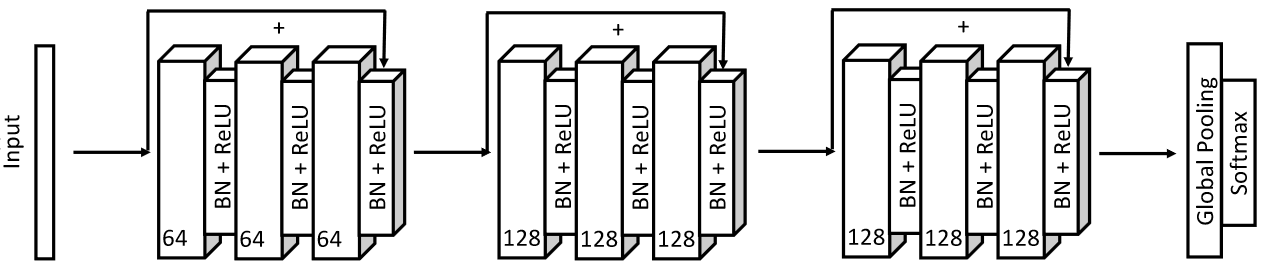
\includegraphics[width=\textwidth]{figures/impl_ResNet11.png}
        \caption{\acrfull{resnet11}}
        \source{\textcite{wang2016}}
        \label{fig:impl_ResNet11}
    \end{subfigure}
    \begin{subfigure}[b]{\textwidth}
        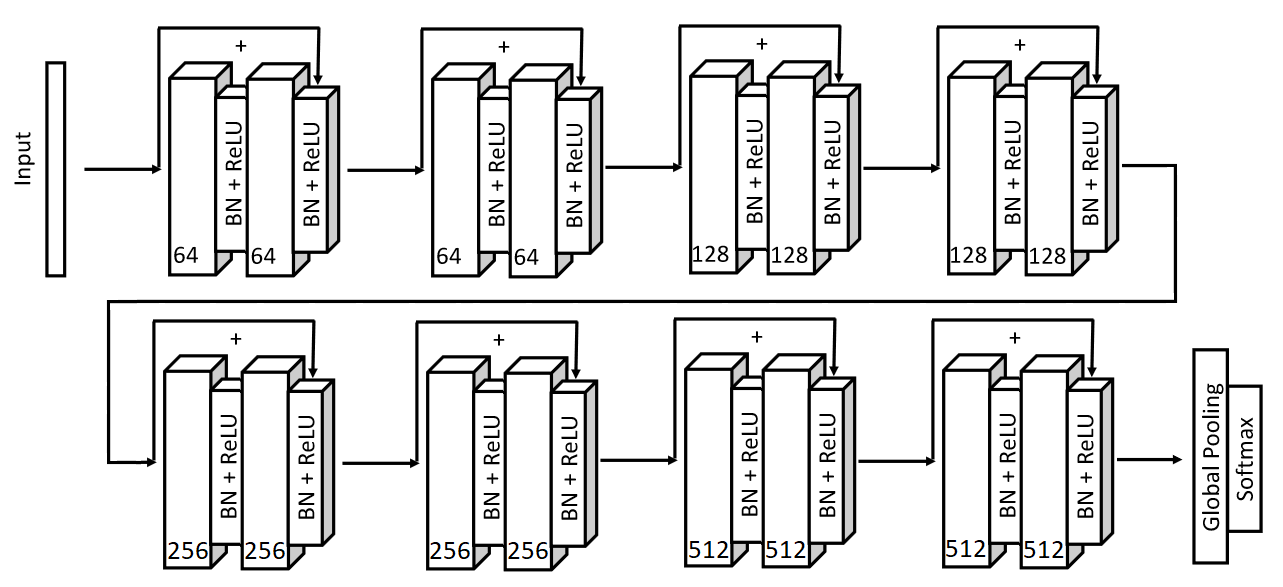
\includegraphics[width=\textwidth]{figures/impl_ResNet18.png}
        \caption{\acrfull{resnet18}}
        \label{fig:impl_ResNet18}
    \end{subfigure}
    \caption{Model architectures of \acrshort{resnet11} and \acrshort{resnet18}. Three dimensional layers represent convolutions, numbered by filter count. Characteristic to ResNet architectures is the "skip-connections" represented by arrows skipping every two- or three convolutional blocks.}
\end{figure}

The two final models presented in this thesis are based on an architecture made famous for computer vision by \textcite{he2015}, known as Residual Networks. At the time, a complication that was known as "the vanishing gradient problem"  plagued most architectures of any considerable depth. It was caused due to the iterative training approach described in section \ref{sec:bt/DNN}, where weights of the network are updated according to the gradient of the error function with respect to each weight. For every added layer, the gradients are multiplied, eventually approaching zero. In the worst case, this may slow and even halt the training process entirely \cite{basodi2020}. Residual Networks solve this problem by introducing \textit{skip connections} that allow for gradients to flow past convolutions from start to end. This architecture won several image classification competitions after its inception in 2015, and skip connections have been employed in many other state-of-the-art model architectures since.

In the original paper, \textcite{he2015} introduced five distinct ResNet architectures, ranging from 18 to 152 layers in depth. However, to avoid comparing models with over an order of magnitude of difference in depth, the architecture used here will be limited to an \acrfull{resnet18}. This architecture employs eight \textit{ResNet blocks}, each including two convolutional layers followed by a batch normalization layer activated by \acrshort{relu}. The input to every ResNet block is saved and added to its output, which constitutes a skip connection. Internal convolutional layers use an increasing amount of filters over the depth of the network, from 64 to 512 filters. Just like the \acrshort{fcn}, the outputs from the convolutional filters are sent through a global average pooling which collapses their time dimension. Finally, a fully-connected layer activated by softmax ensures a probability distribution over classes.

A modification to the original ResNet architectures was proposed by \textcite{wang2016}. This version, an \acrfull{resnet11}, has proven to be accurate on \acrshort{tsc}, and is presented in figure \ref{fig:impl_ResNet11}. Contrary to \acrshort{resnet18}, this version consists of three larger ResNet blocks, each with three convolutional layers employing 64, 128, and 128 filters. Otherwise, the input, output, and skip connections of this architecture are similar to that of \acrshort{resnet18}.

Both ResNet architectures sport the greatest of parameters of all convolutional models detailed and developed in this thesis. Their complexity is expected to influence the training process significantly. \acrshort{resnet11} has $522,756$ parameters, while the deeper and more complex \acrshort{resnet18} sports as much as $4,190,084$. 

% Both ResNet versions possess similar advantages as the \acrshort{fcn}, having a number of parameters which is invariant of the size of its inputs.

% \newpage
% \subsection{Hyperparameters and Training}

% In addition to comparing the intrinsically different architectures detailed above, the classifications each model produces are highly influenced by the parameters with which they are trained. Some mostly affected training efficiency, while others had a clear effect on either classification accuracy or tendency to overfit the training data.

% \begin{itemize}
%     \item Segment length
%     \item Time series augmentation
%     \item Blink rate attention window
%     \item Time series smoothing window
%     \item ? Batch size
%     \item ? Learning rate
%     \item ? Dropout
%     \item Batch Normalization
% \end{itemize}